% Fachvortrag - Evolutionsstrategien - Jannis Weber + Niklas Hartinger - Praktikum Künstliche Intelligenz
\documentclass[%
	BCOR=8.25mm,         % Bindekorrektur
	DIV=12,              % Satzspiegel
	parskip=half,				 % Abstand zwischen Absätzen
	bibliography=totoc,	 % Literaturverzeichnis im Inhaltsverzeichnis
	headsepline=on,      % Trennlinie Kolumnentitel
	cleardoublepage=plain % page numbers on standard cleared double pages
	]{scrartcl}

%% Präambel
\usepackage[english, ngerman]{babel} % deutsche typogr. Regeln + Trenntabelle
\usepackage[T1]{fontenc}             % interner TeX-Font-Codierung
\usepackage{lmodern}                 % Font Latin Modern
\usepackage[utf8]{inputenc}          % Font-Codierung der Eingabedatei
\usepackage[babel]{csquotes}         % Anführungszeichen
\usepackage{graphicx}                % Graphiken
\usepackage{booktabs}                % Tabellen schöner
\usepackage{listingsutf8}            % Listings mit Einstellungen
\lstset{basicstyle=\small\ttfamily,
	tabsize=2,
	basewidth={0.5em,0.45em},
	extendedchars=true}
\usepackage{amsmath}	               % Mathematik
\usepackage[pdftex]{hyperref}
\hypersetup{
	bookmarksopen=true,
	bookmarksopenlevel=3,
	colorlinks=true,
	citecolor=black,
	linkcolor=black,
	urlcolor=magenta
}
\usepackage{scrhack}								 % unterdrückt Fehlermeldung von listings

%% Verzeichnisse
\usepackage{tocstyle} 
\usetocstyle{KOMAlike}

%% Nummerierungstiefen
\setcounter{tocdepth}{3}             % 3 Stufen im Inhaltsverzeichnis
\setcounter{secnumdepth}{3} 		     % 3 Stufen in Abschnittnummerierung




% CUSTOM ADDED PACKAGES START HERE

\usepackage{float}
\usepackage{caption}
\usepackage{subcaption}
%\usepackage[automake, acronym]{glossaries}
\usepackage{tabulary}
\usepackage{tikz}
\usepackage{listings}
\usepackage{color}
\usepackage{pdflscape}
\usepackage{tocloft}
\usepackage{amssymb}
\usepackage{xurl}

\usepackage[nottoc]{tocbibind}

% use equal fonts
\usepackage[scaled=.92]{helvet}
\usepackage{fancyhdr}

% fixes capitalization of header of bibliography
\fancypagestyle{bibliography}{%
  \renewcommand{\headrulewidth}{0.4pt}% reset to original width
  \fancyhf{}%
  \fancyhead[LE]{\fontfamily{ptm}\fontseries{m}\slshape\fontsize{11}{14}\selectfont Literaturverzeichnis}%
  \fancyhead[RO]{\fontfamily{ptm}\fontseries{m}\slshape\fontsize{11}{14}\selectfont Literaturverzeichnis}%
  \fancyfoot[LE]{\thepage}%
  \fancyfoot[RO]{\thepage}%
}

% keep page numbers for zusammenfassung, eidesstattliche erklärung und sperrvermerk
\fancypagestyle{entrypage}{%
  \renewcommand{\headrulewidth}{0pt}%
  \fancyhf{}%
  \fancyfoot[CE]{\thepage}%
  \fancyfoot[CO]{\thepage}%
}

\fancypagestyle{finalpage}{%
  \renewcommand{\headrulewidth}{0.4pt}% reset to original width
  \renewcommand{\headwidth}{30cm}% reset to original width
  \fancyhf{}%
  \fancyfoot[LE]{\hfill\hfill\thepage}%
  \fancyfoot[RO]{\hfill\hfill\thepage}%
}

% remove footnote counter reset after every section
%\counterwithout{footnote}{section}

\usepackage[hyperpageref]{backref}
\renewcommand*{\backref}[1]{}
\renewcommand*{\backrefalt}[4]{%
    \ifcase #1 [nicht zitiert]%
    \or        [zitiert auf Seite~#2]%
    \else      [zitiert auf Seite~#2]%
    \fi}
\backrefgerman

%\makeglossaries
%\loadglsentries{glossary}
%\loadglsentries{acronyms}

\lstset{literate=%
{Ö}{{\"O}}1
{Ä}{{\"A}}1
{Ü}{{\"U}}1
{ß}{{\ss}}2
{ü}{{\"u}}1
{ä}{{\"a}}1
{ö}{{\"o}}1
}

% fix old fonts
\makeatletter
\DeclareOldFontCommand{\rm}{\normalfont\rmfamily}{\mathrm}
\DeclareOldFontCommand{\sf}{\normalfont\sffamily}{\mathsf}
\DeclareOldFontCommand{\tt}{\normalfont\ttfamily}{\mathtt}
\DeclareOldFontCommand{\bf}{\normalfont\bfseries}{\mathbf}
\DeclareOldFontCommand{\it}{\normalfont\itshape}{\mathit}
\DeclareOldFontCommand{\sl}{\normalfont\slshape}{\@nomath\sl}
\DeclareOldFontCommand{\sc}{\normalfont\scshape}{\@nomath\sc}
\makeatother

% removes indentation of paragraphs at the start of a paragraph
\setlength{\parindent}{0pt}
% removes automatic spacing between paragraphs if page is not filled
\raggedbottom

%%% % Hurenkinder und Schusterjungen verhindern
%%% \clubpenalty = 10000 % schliesst Schusterjungen aus 
%%% \widowpenalty = 10000 \displaywidowpenalty = 10000 % schliesst Hurenkinder aus
%%% \widowpenalties=3 10000 10000 10000
% Hyphenpenalty
%%% %\usepackage[none]{hyphenat}
%%% %\righthyphenmin 10000
%%% %\hyphenchar\font=-1
\tolerance=1
\emergencystretch=\maxdimen
\hyphenpenalty=10000
\hbadness=10000

\usepackage{float}

\lstset{literate=%
{Ö}{{\"O}}1
{Ä}{{\"A}}1
{Ü}{{\"U}}1
{ß}{{\ss}}2
{ü}{{\"u}}1
{ä}{{\"a}}1
{ö}{{\"o}}1
}

\definecolor{lightgray}{rgb}{.9,.9,.9}
\definecolor{darkgray}{rgb}{.4,.4,.4}
\definecolor{purple}{rgb}{0.65, 0.12, 0.82}
\definecolor{darkgreen}{rgb}{0,.4,0}

\lstdefinelanguage{TypeScript}{
  keywords={await, typeof, new, true, false, catch, function, return, null, catch, switch, var, const, let, if, in, while, do, else, case, break, async, static},
  keywordstyle=\color{blue}\bfseries,
  ndkeywords={class, export, throw, implements, import, this},
  ndkeywordstyle=\color{darkgray}\bfseries,
  identifierstyle=\color{black},
  sensitive=false,
  comment=[l]{//},
  morecomment=[s]{/*}{*/},
  commentstyle=\color{purple}\ttfamily,
  stringstyle=\color{red}\ttfamily,
  morestring=[b]',
  morestring=[b]"
}

\newcommand{\setlistingtotypescript}[0]{
\lstset{
   language=TypeScript,
   backgroundcolor=\color{lightgray},
   extendedchars=true,
   basicstyle=\ttfamily\large,
   showstringspaces=false,
   showspaces=false,
   numbers=left,
   numberstyle=\footnotesize,
   numbersep=9pt,
   tabsize=2,
   breaklines=true,
   showtabs=false,
   captionpos=b,
   classoffset=1,
   sensitive=true,
   morekeywords={boolean, Boolean, number, Number, string, ITransportProfile, RoutingProfile, BuildingSetup, ILocation, Region, ICompound, PartialRoute, IPath, ORSResult, IPathResult},
   keywordstyle=\color{darkgreen},
   escapeinside=\$\$
}
}

\newcommand{\setlistingtocpp}[0]{
\lstset{
	language=C++,
	backgroundcolor=\color{lightgray},
	extendedchars=true,
	basicstyle=\ttfamily\large,
	showstringspaces=false,
	showspaces=false,
	numbers=left,
	numberstyle=\footnotesize,
	numbersep=9pt,
	tabsize=2,
	breaklines=true,
	showtabs=false,
	captionpos=b,
    keywordstyle=\color{blue},
	escapeinside=\$\$
}
}

\newcommand{\setlistingtosql}[0]{
\lstset{
	language=SQL,
	backgroundcolor=\color{lightgray},
	extendedchars=true,
	basicstyle=\ttfamily\large,
	showstringspaces=false,
	showspaces=false,
	numbers=left,
	numberstyle=\footnotesize,
	numbersep=9pt,
	tabsize=2,
	breaklines=true,
	showtabs=false,
	captionpos=b,
	morekeywords={int, varchar, double, tinyint, bigint, unsigned, REFERENCES, ENGINE, CHARSET, COMMENT},
	keywordstyle=\color{blue},
	escapeinside=\$\$,
}
}

\newcommand{\setlistingtopseudocode}[0]{
\lstset{
  	backgroundcolor=\color{lightgray},
  	extendedchars=true,
   	basicstyle=\ttfamily\large,
   	showstringspaces=false,
   	showspaces=false,
   	numbers=left,
   	numberstyle=\footnotesize,
   	numbersep=9pt,
   	tabsize=4,
   	breaklines=true,
   	showtabs=false,
   	captionpos=b,
   	classoffset=1,
   	sensitive=true,
   	mathescape=true,
   	escapeinside={<@}{@>}
}
}

\newcommand{\colorcodeline}[1]{\textcolor{blue}{#1}}

\newcommand{\colorcodealgorithm}[1]{\textcolor{darkgreen}{#1}}

% for repeating a figure without being included in the list of figures
\newcommand{\repeatcaption}[2]{%
  \renewcommand{\thefigure}{\ref{#1}}%
  \captionsetup{list=no}%
  \caption{#2 (von Seite \pageref{#1})}%
  \addtocounter{figure}{-1}
}

% define fix usage of \Leftrightarrow, use as \noleftright
\newcommand{\notleftright}{\mathrel{\ooalign{$\Leftrightarrow$\cr\hidewidth$/$\hidewidth}}}

\DeclareCaptionType{equ}[][]
\makeatletter
\def\l@lstlisting#1#2{\@dottedtocline{1}{1.5em}{3em}{#1}{#2}}
\makeatother

% pulls section start upwards
%\RedeclareSectionCommand[beforeskip=0pt, afterskip=0.5cm]{section}

% see: https://tex.stackexchange.com/questions/161327/how-to-flip-even-odd-page-style
\let\tempmargin\oddsidemargin
\let\oddsidemargin\evensidemargin
\let\evensidemargin\tempmargin
\reversemarginpar

%--- ---%
% use \raggedbottom or \vfill to correct text placement if text was moved weirdly
%--- ---%

% ----------------------------------------------------------------------------
\begin{document}

\pagenumbering{Roman}

%% Titelseite
\begin{titlepage}
	\begin{center}
	
\includegraphics[width=0.9\textwidth]{img/mni-logo}
	
	\vspace{3cm}	

	\huge\textbf{\sffamily Ausarbeitung Projektvortrag}

	\vspace{1cm}	

	\Huge\textbf{\sffamily Genetische Algorithmen}

	\normalsize
	\vspace{1cm}

	von \\[1cm]	

	\Huge\textbf{Niklas Hartinger}\\ [.5cm]\normalsize
	Matrikelnummer: 5183113\\ [.75cm]
	
	und \\[1cm]	
	
	\LARGE\textbf{Jannis Weber}\\ [.5cm]\normalsize
	Matrikelnummer: 5204678\\ [.75cm]
	
	im Januar 2021
	\end{center}
	\vfill
	\begin{tabular}{ll}
		Dozent: & Professor Dr. Wolfgang Henrich 
	\end{tabular}
\end{titlepage}

%% Zusammenfassung
\pagestyle{entrypage}
% reset page to 1
\setcounter{page}{1}
\begin{quote}
	\vspace*{4cm}

	\begin{center}
		\textbf{\Large\sffamily Zusammenfassung}
	\end{center}
	\vspace*{.5cm}
	
\end{quote}

	Evolutionsstrategien gehören zu den Evolutionären Algorithmen und dienen als Modellierung der biologischen Evolution.\\
	Mit unterschiedlich komplexen Parameterkombinationen lassen sich Optimierungsprobleme lösen, indem eine sukzessive Annäherung an die optimale Lösung mithilfe der Evolutionsschritte erreicht wird.\\
	In dieser fachlichen Ausarbeitung wird die Funktionsweise der wesentlichen Evolutionsstrategien sowie deren Kernaspekte ausgearbeitet und anschließend mit den allgemeinen Genetischen Algorithmen verglichen.\\
	Abschließend wird das Problem des Handlungsreisenden aufgegriffen, welches es anhand der erlernten Inhalte in einem praxisorientierten Projekt zu bearbeiten gilt.
	
\phantomsection
\addcontentsline{toc}{section}{Zusammenfassung}
\cleardoublepage

%% Verzeichnissse
%\settocfeature{entryhook}{\sffamily}    % alle Einträge wie im Text serifenlos
\tableofcontents
\cleardoublepage

\settocfeature{entryhook}{\rmfamily}    % Einträge wie im Text mit Serifen

\listoffigures
% durch \usepackage[nottoc]{tocbibind} nicht mehr notwendig
%\phantomsection
%\addcontentsline{toc}{section}{\listfigurename}
\cleardoublepage

\listoftables
% durch \usepackage[nottoc]{tocbibind} nicht mehr notwendig
%\phantomsection
%\addcontentsline{toc}{section}{\listtablename}
\cleardoublepage

\renewcommand\lstlistingname{Code-Listing}
\renewcommand\lstlistlistingname{Code-Listings}
\lstlistoflistings
\phantomsection
\addcontentsline{toc}{section}{\lstlistlistingname}
\cleardoublepage

\newcommand{\listequationsname}{Formelsammlung}
\newlistof{myequations}{equ}{\listequationsname}
\newcommand{\myequations}[1]{%
	\addcontentsline{equ}{section}{\protect\numberline{\theequation}#1}\par
}
\listofmyequations
\phantomsection
\addcontentsline{toc}{section}{\listequationsname}
\cleardoublepage

% Abstand im Inhaltsverzeichnis
\addtocontents{toc}{\vspace{\normalbaselineskip}}

\cleardoublepage

\pagenumbering{arabic}

% KAPITEL HIER EINFÜGEN
\setlistingtopseudocode
\include{einführung}
%-- einleitung

\section{Konzept}

\subsection{Anforderungsanalyse}

\subsection{Systemmodellierung}

\begin{figure}[H]
\centering
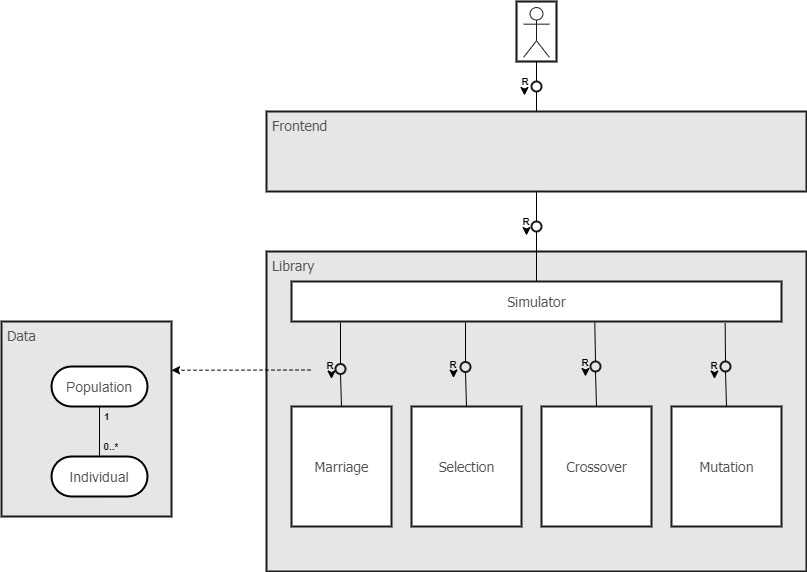
\includegraphics[width=1\textwidth]{img/Vortrag/Systemmodellierung.png}
\caption{Systemmodellierung}
\label{fig:systemmodellierung}
\end{figure}

%--
%-- einleitung

\section{Projektumsetzung}
In diesem Abschnitt wird beschrieben, wie das Konzept umgesetzt wurde.
Es wird erläutert, für welche Programmteile welche Programmiersprachen eingesetzt werden. Darüber hinaus wird der Einsatz von Fremdbibliotheken aufgezeigt.
Anschließend wird mit Hilfe von  Programmcode-Ausschnitten die Implementierung der Genetischen Algorithmen erklärt.

\subsection{Programmiersprachen}
Durch die Trennung von Frontend und der Library ergeben sich für diese beiden Programmteile unterschiedliche Anforderungen an die Programmiersprache.\\
Die Library setzt die Genetischen Algorithmen um, die während einer Simulation mehrere tausend Berechnungen durchführt. Für diesen Zweck wurde sich für die Programmiersprache C++ entschieden.
Dabei handelt es sich um eine maschinennahe Sprache mit hohen Ausführungsgeschwindigkeiten. Allerdings ist die Entwicklung mit C++ sehr zeitaufwendig. Dadurch, dass es sich bei der Library um den zeitkritischen Teil des Projektes handelt, 
wurde sich trotz des hohen Aufwands für diese Programmiersprache entschieden.\\
Das Frontend hingegen soll lediglich die Verwendung der Library demonstrieren. In diesem Fall steht eine hohe Entwicklungsgeschwindigkeit im Vodergrund und deshalb wurde sich für Python als Frontend-Programmiersprache  entschieden. 
Diese interpretierte Sprache ist im Vergleich zu C++ langsamer, ermöglicht aber eine schnellere und unkompliziertere Enwicklung.

\subsection{Frameworks und Bibliotheken}
Eine Übersicht über die verwendeten Bibliotheken ist in Tabelle \ref{tab:bibs} zu sehen.\\
Zur Entwicklung der Library für die Genetischen Algorithmen war ein Testsystem notwendig. Mit automatisierten Test wird sichergestellt, dass entwickelter Code die angedachten Aufgaben korrekt erfüllt.
Für diesen Zweck wurde die C++ Bibliothek Catch2 eingesetzt. Bei Catch2 handelt es sich um eine sogenannte Single-Header-Library. Das bedeutet, dass der gesamte Bibliothekscode in einer Datei zu finden ist.
Dadurch war eine sehr einfache Einbindung in das Projekt möglich. Catch2 läuft unter der Boost-Software-License, was eine kostenlose Nutzung der Bibliothek ermöglicht.\\
Des weiteren wurde eine Bibliothek zum visualisieren von Simualtionsergebnissen eingesetzt. Dazu wurde die sehr beliebte Matplotlib verwendet. Diese ermöglicht das einfache erstellen von Graphen in Python aber auch C++.
In diesem Projekt wurde Matplotlib nur auf der Python-Seite verwendet. Die Biliothek läuft unter der Matplotlib-License, bei der es sich um eine Open-Source-Lizens handelt.\\
Damit ein Python Programm überhaupt C++ Code ausführen kann, ist es notwenig Schnittstellen von C++ zu Python bereitzustellen. Dafür wurde das Python-Modul der Boost-Bibliothek verwendet. Mit diesem war eine sehr schnelle Schnittstellenentwicklung möglich.
Auch die Boost-Bibliothek läuft unter der Boost-Software-Lizence und ist dadurch für eine kostenlose Nutzung freigegeben.
\begin{table}
\caption{Verwendeten Bibliotheken}
\begin{tabular}{|l|l|l|l|}
 Name & Version & Anwendung & Lizenz \\ 
\hline
 Catch2 & 2.13 & Unit-Tests der Library & Boost Software License \\  
 Matplotlib & 3.2 & Visualisierung der Experimente & Matplotlib License \\
 Boost & 1.7 & Schnittstelle zwischen C++ und Python & Boost Software License    
\end{tabular}
\label{tab:bibs}
\end{table}

\subsection{Individuen und Populationen}
Wie in der Systemmodellieung \ref{fig:systemmodellierung} zu sehen war, verarbeiten die Genetischen Algorithmen Individuen und Populationen. Aus diesem Grund wurden diese beiden Objekttypen als Klasse implementiert. Das dazugehörige Klassendiagramm ist in Abbildung \ref{fig:klassendiagramm} zu sehen.
Die Individuen speichern dabei die Chromosome als ganzzahlige Liste. In dieser Liste sind die Routeninformationen gespeichert. Es wurde sich dafür entschieden die Route als eine Liste von nacheinander besuchten Stadtindezes zu implementieren. Die Startstadt ist allerdings kein Teil dieser Liste, weil sich diese bei den Verarbeitungsschritten nicht verändern soll.
Der Vorteil dieser Codierung ist eine leichte Überprüfbarkeit der TSP-Vorgabe, dass jede Stadt nur einmal besucht werden darf. Es muss lediglich berechnet werden, dass jede Stadt, außer der Startstadt, innerhalb der Liste genau einmal vorkommt. Diese Validierungsfunktionalität ist in der Methode is\_valid() des Individuums implementiert.
Hätte man sich für eine binäre Codierung entschieden, bei der die Bitposition angibt, welche Verbindungen besucht wurden, dann wäre eine solche Überprüfung deutlich komplizierter.\\
Ein Individuum benötigt für die Verarbeitung innerhalb der Genetischen Algorithmen eine Fitness- und eine Bewertungsfunktion. Die Bewertungsfunktion berechnet, wie nah ein Individuum an einem optimalen Individuum liegt und die Fitnessfunktion entspricht der Wahrscheinlichkeit als Elternindividuum ausgewählt zu werden.
Es wurde sich dafür entschieden, dass ein Individuum seine Fitness- und Bewertungsfunktion bei der Objekterstellung übergeben bekommt. Somit wird ermöglicht diese Funktionen sehr schnell auszutauschen. Die Funktionen fitness und rating des Individuums verwenden anschließend lediglich diese injizierten Funktionen.\\
Eine Menge an Individuuen bildet eine Population. Eine Populationen wird dazu eingesetzt unkompliziert mit vielen Individuen zu arbeiten. Dazu bietet diese Klasse die Funktionalität die Fitness aller enthaltenen Individuen zu berechne, das fitteste und unfitteste Individuum zurückzugeben und die Menge an Individuuen zu aktualisieren.
Darüber hinaus speichert die Population die Startstadt und die Distanzdaten. Diese sind zur Berechnung der Fitness und Bewertung der Individuen notwendig.
\begin{figure}[H]
\centering
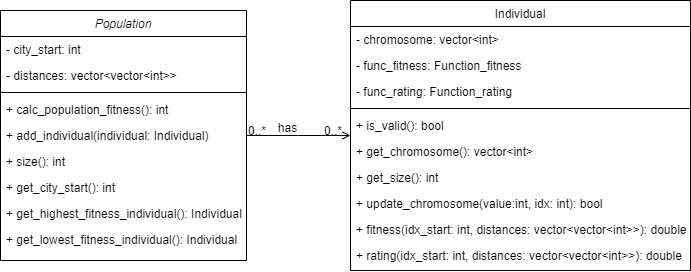
\includegraphics[width=1\textwidth]{img/Vortrag/uml.png}
\caption{Klassendiagramm Individuum und Population}
\label{fig:klassendiagramm}
\end{figure}


\subsection{Bewertungs und Fitnessfunktion}
In Listing \ref{lst:rating} ist eine Bewertungsfunktion zu sehen, die in diesem Projekt verwendet wurde. Diese berechnet die Bewertung eines Chromosoms mit Hilfe einer Distanzmatrix. In Zeile 4 wird die Distanz von der Startstadt zur ersten Stadt innerhalb des Chromosoms bestimmt. Anschließend werden von Zeile 5 bis 9 alle Distanzen des Chromosoms hinzugerechnet. Als letztes wird in Teile 10 die Verbindung der letzten Stadt im Chromosom zur Startstadt addiert. Somit ist die Bewertung die Gesamtdistanz der Route und die funktionale Anforderung 3FA ist erfüllt. Diese Distanz soll innerhalb des Verfahrens minimiert werden.\\
In Listing \ref{lst:fitness} ist die Fitnessfunktion zu sehen, die in diesem Projekt verwendet wurde. Diese negiert lediglich die berechneten Bewertungen der Individuen. Damit wird erreicht, dass ein Individuum mit einer niedrigen Gesamtdistanz als fitter angesehen wird als ein Individuum mit hoher Gesamtdistanz.

\begin{minipage}{\linewidth}
\begin{lstlisting}[caption={Beispiel einer Ratingfunktion}, firstnumber=1, captionpos=b, label=lst:rating]
double func_rating(int idx_start, vector<int> chromosome, vector<vector<int>> distances){
	int city_a, city_b;
	int rating = 0;
	costs += get_distance(idx_start, chromosome.at(0), distances);
	for (unsigned int i = 0; i < chromosome.size() - 1; ++i) {
		city_a = chromosome.at(i);
		city_b = chromosome.at(i + 1);
		rating += get_distance(city_a, city_b, distances);
	}
	rating += get_distance(chromosome.at(chromosome.size() - 1), idx_start, distances);
	return rating;
}
\end{lstlisting}
\end{minipage}
\begin{minipage}{\linewidth}
\begin{lstlisting}[caption={Beispiel einer Fitnessfunktion}, firstnumber=1, captionpos=b, label=lst:fitness]
double func_fitness(double rating){
	return -rating;
}
\end{lstlisting}
\end{minipage}
\subsection{Marriage-Algorithmus}
\begin{minipage}{\linewidth}
\begin{lstlisting}[caption={Marriage-Roulette Algorithmus}, firstnumber=1, captionpos=b, label=lst:marriage]
pair<int, int> marriage_roulette_reversed(Population &population) {
	pair<int, int> pair = make_pair(-1, -1);
	int sum = 0;
	int worst_fitness_of_population = (int) population.get_lowest_fitness_individual().get_last_calculates_fitness();
	for (auto &it : population.get_individuals()) {
		sum += (int) it.get_last_calculates_fitness() - worst_fitness_of_population;
	}
	int value_p1 = random(sum);
	int value_p2 = random(sum);

	int value = 0;
	for (unsigned int current_idx = 0; current_idx < population.size(); ++current_idx) {
		value += (int) population.get_individuals().at(current_idx).get_last_calculates_fitness() - worst_fitness_of_population;
		if (value_p1 <= value && pair.first < 0) {
			pair.first = current_idx;
		}
		if (value_p2 <= value && pair.second < 0) {
			pair.second = current_idx;
		}
	}
	return pair;
}
\end{lstlisting}
\end{minipage}
\begin{center}
\begin{tabular}{|l|l|l|}
 Individuum & Fitness & Delta \\ 
\hline
 1 & -1180 & 820 \\  
 2 & -1680 & 320 \\  
 3 & -1860 & 140 \\  
 4 & -1880 & 120 \\  
 5 & -2000 & 0 \\  
\end{tabular}
\end{center}

\subsection{Crossover-Algorithmen}

\subsubsection{Partialliy-Matched-Crossover}
\begin{minipage}{\linewidth}
\begin{lstlisting}[caption={Partially-Matched-Crossover}, firstnumber=1, captionpos=b, label=lst:pmx]
void partially_matched_crossover(Individual &p1, Individual &p2, Individual &c1, Individual &c2) { 
	int length = p1.get_size();
	int interval_border_left, interval_border_right = calc_two_random_interval_borders(length);

	for (int i = 0; i < length; ++i) {
		if (i < interval_border_left || i >= interval_border_right) {
			c1.update_chromosome(p1.get_chromosome().at(i), i);
			c2.update_chromosome(p2.get_chromosome().at(i), i);
		} else {
			c1.update_chromosome(p2.get_chromosome().at(i), i);
			c2.update_chromosome(p1.get_chromosome().at(i), i);
		}
	}

	duplicate_correction_pmx(p1, p2, c1);
	duplicate_correction_pmx(p2, p1, c2);
}
\end{lstlisting}
\end{minipage}
\subsubsection{Order-Crossover}
\begin{minipage}{\linewidth}
\begin{lstlisting}[caption={Order-Crossover}, firstnumber=1, captionpos=b, label=lst:ox]
void order_crossover(Individual &p1, Individual &p2, Individual &c1, Individual &c2) {
	int length = p1.get_size();
	int interval_border_left, interval_border_right = calc_two_random_interval_borders(length);

	unordered_map<int, int> map_p1, map_p2;
	for (int i = interval_border_left; i < interval_border_right; ++i) {
		map_p1.insert(pair<int, int>(p1.get_chromosome().at(i), i));
		map_p2.insert(pair<int, int>(p2.get_chromosome().at(i), i));
	}
	vector<int> cache1, cache2;
	set_duplicate_flags(map_p2, c1, p1, cache1, interval_border_left, interval_border_right);
	set_duplicate_flags(map_p1, c2, p2, cache2, interval_border_left, interval_border_right);
	copy_values(c1, cache1, interval_border_left);
	copy_values(c2, cache2, interval_border_left);

	for (int j = interval_border_left; j < interval_border_right; ++j) {
		if (c1.get_chromosome().at(j) == DUPLICATE_FLAG) {
			c1.update_chromosome(p2.get_chromosome().at(j), j);
		}
		if (c2.get_chromosome().at(j) == DUPLICATE_FLAG) {
			c2.update_chromosome(p1.get_chromosome().at(j), j);
		}
	}
}
\end{lstlisting}
\end{minipage}
\subsubsection{Cycle-Crossover-One-Cycle}
\begin{minipage}{\linewidth}
\begin{lstlisting}[caption={Cycle-Crossover-One-Cycle}, firstnumber=1, captionpos=b, label=lst:cxo]
void cycle_crossover_one_cycle(Individual &p1, Individual &p2, Individual &c1, Individual &c2) {
	vector<bool> index_flags(p1.get_size(), false);
	Cycle cycle;
	int cycle_start_idx = random(p1.get_size());
	fill_empty_cycle_with_tuples(cycle, cycle_start_idx, p1, p2, index_flags)
	int tupleCounter = 0;
	for (int i = 0; (unsigned int) i < index_flags.size(); ++i) {
		bool flag = index_flags.at(i);
		if (flag) {
			Tuple &t = cycle.at(tupleCounter);
			tupleCounter++;
			c1.update_chromosome(get<1>(t), get<0>(t));
			c2.update_chromosome(get<2>(t), get<0>(t));
		} else {
 			c1.update_chromosome(p2.get_chromosome().at(i), i);
			c2.update_chromosome(p1.get_chromosome().at(i), i);
		}
	}
}
\end{lstlisting}
\end{minipage}

\subsubsection{Cycle-Crossover-All-Cycles}
\begin{minipage}{\linewidth}
\begin{lstlisting}[caption={Cycle-Crossover-All-Cycles}, firstnumber=1, captionpos=b, label=lst:cxa]
void cycle_crossover_all_cycles(Individual &p1, Individual &p2, Individual &c1, Individual &c2) {
	vector<bool> index_flags(p1.get_size(), false);
	vector<Cycle> cycles;
	for (int cycle_start_idx = 0; cycle_start_idx < p1.get_size(); ++cycle_start_idx) {
		Cycle cycle;
		if (!index_flags.at(cycle_start_idx)) {
			fill_empty_cycle_with_tuples(cycle, cycle_start_idx, p1, p2, index_flags)
		}
		cycles.push_back(cycle);
		}
	}
	for (int i = 0; (unsigned int) i < cycles.size(); ++i) {
		bool cross_copy = i % 2 != 0;
		Cycle &cycle = cycles.at(i);
		for (Tuple &t : cycle) {
			if (cross_copy) {
				c1.update_chromosome(get<2>(t), get<0>(t));
				c2.update_chromosome(get<1>(t), get<0>(t));
			} else {
				c1.update_chromosome(get<1>(t), get<0>(t));	
 				c2.update_chromosome(get<2>(t), get<0>(t));
			}
		}
	}
}

\end{lstlisting}
\end{minipage}
\subsubsection{Edge-Recombination-Crossover}
\begin{minipage}{\linewidth}
\begin{lstlisting}[caption={Edge-Recombination-Crossover}, firstnumber=1, captionpos=b, label=lst:erx]
bool edge_recombination_crossover(Individual &p1, Individual &p2, Individual &c1, Individual &c2) {
	map<int, set<int>> edge_map = create_edge_map(p1, p2);
	edge_recombination(p1.get_chromosome().at(0),c1, edge_map);
	edge_recombination(p2.get_chromosome().at(0),c2, edge_map);
	return true;
}

void edge_recombination(int start, Individual &i, map<int, set<int>> edge_map) {
	int current = start;
	for (int idx = 0; idx < i.get_size() - 1; ++idx) {
		i.update_chromosome(current, idx);
		for (auto &it : edge_map) {
			it.second.erase(current);
		}
		int min_next_idx = -2;
		unsigned int min_next_count = numeric_limits<int>::max();

		for (int node : edge_map.at(current)) {
			if (edge_map.at(node).size() < min_next_count) {
				min_next_count = edge_map.at(node).size();
				min_next_idx = node;
			}
		}
		current = min_next_idx;
		if (idx == i.get_size() - 2) {
			i.update_chromosome(current, idx + 1);
		}
	}
}
\end{lstlisting}
\end{minipage}

\subsection{Mutations-Algorithmus}
\begin{minipage}{\linewidth}
\begin{lstlisting}[caption={Delete-Shift-Mutaions-Algorithmus}, firstnumber=1, captionpos=b, label=lst:mutation]
bool mutation_delete_shift(Individual &individual, int percentage) {
	bool mutate = rand(100)  < percentage;
	if (mutate) {
		int position_a = rand(individual.get_size() - 1);
		int position_b = rand(position_a + 1, individual.get_size());
 
		for (int i = position_a; i < position_b; i++) {
			swap_chromosome(individual.get_chromosome(), i, i + 1);
		}
	}
	return mutate;
}
\end{lstlisting}
\end{minipage}
\subsection{Selektions-Algorithmus}
\begin{minipage}{\linewidth}
\begin{lstlisting}[caption={Survival-Of-The-Fittest-Selektions-Algorithmus}, firstnumber=1, captionpos=b, label=lst:selektion]
Population selection_sotf(Population &p_old, Population &p_new) {
	int size = (int) p_old.size();
	p_old.calc_population_fitness();
	p_new.calc_population_fitness();
	Population result = Population(p_old.get_idx_start(), p_old.get_distances());

	vector<Individual> individuals_old = p_old.get_individuals();
	vector<Individual> individuals_new = p_new.get_individuals();

	sort(individuals_new.rbegin(), individuals_new.rend());
	sort(individuals_old.rbegin(), individuals_old.rend());
	int offset_old = 0;
	int offset_new = 0;
	for (int i = 0; i < size; ++i) {
		if (individuals_old.at(offset_old) < individuals_new.at(offset_new)) {
			result.add_individual(individuals_new.at(offset_new));
			offset_new++;
		} else {
			result.add_individual(individuals_old.at(offset_old));
 			offset_old++;
		}
	}
	return result;
}
\end{lstlisting}
\end{minipage}
\subsection{Simulator}

\begin{figure}[H]
\centering
\includegraphics[width=1\textwidth]{img/Vortrag/simulator.png}
\caption{Klassendiagramm Simulator}
\label{fig:simulator}
\end{figure}

\subsection{Python-Schnittstelle}
\begin{minipage}{\linewidth}
\begin{lstlisting}[caption={C++ zu Python Schnittstelle}, firstnumber=1, captionpos=b, label=lst:boostpython]
BOOST_PYTHON_MODULE(Simulator_Wrapper)
{
	to_python_converter<tuple<int, int, int>, TupleToList<int> >();

	enum_<Selection_Algorithm>("Selection_Algorithm").value("SOTF", Selection_Algorithm::SOTF);

	class_<Simulator>("Simulator", init<
		string, string, string,
		int,int,int,int,
		Crossover_Algorithm, Marriage_Algorithm, Mutation_Algorithm, Selection_Algorithm>(
		))
 		.def("simulate", &Simulator::simulate)
		.def("finished", &Simulator::finished)
		.def("best_individual", &Simulator::best_individual);
}
\end{lstlisting}
\end{minipage}
\subsection{Testen}
\begin{minipage}{\linewidth}
\begin{lstlisting}[caption={Unit-Tests}, firstnumber=1, captionpos=b, label=lst:tests]
SCENARIO("Test Individual initialization", "[Individual.cpp]")
{
	for (int i = 0; i < 100; ++i) {
		Individual individual = Individual(size, idx_start, nullptr, nullptr);
		vector<int> chromosome = individual.get_chromosome();
		REQUIRE(chromosome.size() == (unsigned int) size);
		REQUIRE(unique(chromosome.begin(), chromosome.end()) == chromosome.end());
	}
}
\end{lstlisting}
\end{minipage}
%--
%-- einleitung

\section{Wissenschaftliche Untersuchung}

%--
%-- einleitung

\section{Zusammenfassung}
Im Folgenden werden die Ergebnisse dieser Projektarbeit zusammengefasst, ein Fazit gebildet anschließend mit einem Ausblick die Ausarbeitung beendet.

\subsection{Ergebnisse und Fazit}
Zu Beginn dieser Ausarbeitung wurde beschrieben, welche Ziele zu erreichen sind. Es sollte ein System entwickelt werden, das die Möglichkeiten von Genetischen Algorithmen an dem Beispiel des TSP demonstriert. Für diesen Zweck wurde ein System umgesetzt, das mithilfe einer eigens entwickelten Bibliothek für Genetische Algorithmen Simulationen durchführen kann. In dieser Ausarbeitung wurden zu diesem Zweck die Entwicklungsschritte des Systems dargestellt und wichtige Programmteile ausführlich erläutert. Darunter waren neben Codeausschnitten auch die Beschreibung des Testsystems und der verwendeten Schnittstellen. 
Mit diesem Ansatz konnte ein wiederverwendbares, dokumentiertes und getestetes System entwickelt werden, das die Funktionen der Genetischen Algorithmen leicht nutzbar macht. \\
Nach der Entwicklung des Systems wurde als zweites Ziel definiert, zu untersuchen welche Stellschrauben bei den Genetischen Algorithmen das Resultat inwieweit verbessern beziehungsweise verschlechtern. Dies wurde im Rahmen von Experimenten erreicht. Dabei konnte festgestellt werden, dass bei den Genetischen Algorithmen vor allem die Populationsgröße sowie die Wahl eines geeigneten Crossover-Verfahrens das Ergebnis beeinflusst. Die Mutation nahm bei den Experimenten eine unwichtigere Rolle ein. Mit einem Testdatensatz von 48 Hauptstädten der USA konnte ein Rundlauf nach Vorgaben des TSP generiert werden, der mit lediglich 34373 Meilen 2,4\% schlechter ist als ein optimaler Rundlauf mit 33551 Meilen. \\
Dieses Ergebnis beweist, dass die Genetischen Algorithmen zur Approximierung des Travelling Salesman Problems geeignet sind. Darüber hinaus wurd gezeigt, wie eine Parameteroptimierung durchgeführt werden kann.
\subsection{Ausblick}
Die durchgeführten Experimente erzielten, bei dem gegeben Datensatz, sehr gute Ergebnisse. Es wäre aber auch lohnenswert zu untersuchen, ob ähnlich gute Ergebnisse mit anderen Datensätzen generiert werden können. Ein mögliches Vorgehen wäre es, wenn die Anzahl an Städten größer oder kleiner gewählt wird.
Darüber hinaus wäre es interessant zu untersuchen, ob es Sonderfälle gibt, bei denen die Genetischen Algorithmen mit dem TSP keine guten Ergebnisse erzielen.
%--


% Abstand im Inhaltsverzeichnis
\addtocontents{toc}{\vspace{\normalbaselineskip}}
% automatic bibliography
% \bibliographystyle{plainurl}
\pagestyle{bibliography}
% \bibliography{litverz}
% manual bibliography
%--- Literaturverzeichnis

\begin{thebibliography}{99}

\bibitem{schoeneburg}
	Schöneburg, Eberhard; Heinzmann, Frank; Feddersen, Sven:
	\emph{Genetische Algorithmen und Evolutionsstrategien},
	Sammelwerk,
	1994,
	Addison-Wesley Verlag,
	Bonn,
	ISBN: 978-3-89319-493-3
	
	
\end{thebibliography}

% ---

% \cleardoublepage
\pagestyle{headings}

\end{document}
% ----------------------------------------------------------------------------
